\documentclass[review]{elsarticle}

\usepackage{lineno,hyperref}
\usepackage{pdflscape}
\modulolinenumbers[5]

\journal{Geochimica et Cosmochimica Acta}

%%%%%%%%%%%%%%%%%%%%%%%
%% Elsevier bibliography styles
%%%%%%%%%%%%%%%%%%%%%%%
%% To change the style, put a % in front of the second line of the current style and
%% remove the % from the second line of the style you would like to use.
%%%%%%%%%%%%%%%%%%%%%%%

%% Numbered
%\bibliographystyle{model1-num-names}

%% Numbered without titles
%\bibliographystyle{model1a-num-names}

%% Harvard
\bibliographystyle{model2-names.bst}\biboptions{authoryear}

%% Vancouver numbered
%\usepackage{numcompress}\bibliographystyle{model3-num-names}

%% Vancouver name/year
%\usepackage{numcompress}\bibliographystyle{model4-names}\biboptions{authoryear}

%% APA style
%\bibliographystyle{model5-names}\biboptions{authoryear}

%% AMA style
%\usepackage{numcompress}\bibliographystyle{model6-num-names}

%% `Elsevier LaTeX' style
%\bibliographystyle{elsarticle-num}
%%%%%%%%%%%%%%%%%%%%%%%

\begin{document}

\begin{frontmatter}

\title{Hydrous melting and partitioning in and above the mantle transition zone: insights from water-rich MgO-SiO$_2$-H$_2$O experiments}
%\tnotetext[mytitlenote]{Fully documented templates are available in the elsarticle package on \href{http://www.ctan.org/tex-archive/macros/latex/contrib/elsarticle}{CTAN}.}

%% Group authors per affiliation:
\author{R. Myhill, D. J. Frost}
\address{Bayerisches Geoinstitut, Universit\"{a}t Bayreuth, Universit\"{a}tsstrasse 30, 95447 Bayreuth, Germany}
\cortext[mycorrespondingauthor]{Corresponding author: R. Myhill}
\ead{myhill.bob@gmail.com}

\author{D. Novella}
\address{Laboratoire Magmas et Volcans, Universit\'{e} Blaise Pascal, 5 Rue Kessler, 63038 Clermond-Ferrand, France}

%% or include affiliations in footnotes:
%\author[mymainaddress,mysecondaryaddress]{Elsevier Inc}
%\ead[url]{www.elsevier.com}

%\author[mysecondaryaddress]{Global Customer Service\corref{mycorrespondingauthor}}

%\address[mymainaddress]{1600 John F Kennedy Boulevard, Philadelphia}
%\address[mysecondaryaddress]{360 Park Avenue South, New York}

\begin{abstract}
Hydrous melting at high pressures affects the physical properties, dynamics and chemical differentiation of the Earth. However, probing the compositions of hydrous melts at the conditions of the mantle transition zone has traditionally been challenging. In this study, we conducted high pressure multianvil experiments at 13 GPa between 1200 and 1900 $^{\circ}$C to investigate the liquidus in the system MgO-SiO$_2$-H$_2$O. Water-rich starting compositions were created using platinic acid (H$_2$Pt(OH)$_6$) as a novel water source. As MgO:SiO$_2$ ratios decrease, the T-$X_{H_2O}$ liquidus curve develops an increasingly pronounced concave-down topology. The melting point reduction of enstatite and stishovite at low water contents exceeds that predicted by simple ideal models of hydrogen speciation. We discuss the implications of this work on the behaviour of melts in the deep upper mantle and transition zone, and present new models describing the partitioning of water between the olivine polymorphs and associated hydrous melts. 
\end{abstract}

\begin{keyword}
high pressure \sep mantle \sep hydrous melting \sep water \sep liquidus
\end{keyword}

\end{frontmatter}

\linenumbers

\section{Introduction}
Hydrous melts have a remarkable influence on Earth's surface and interior. Melting at subduction zones is primarily driven by the release of hydrous fluids from the warming slab at about 100 km depth, producing the world's arc volcanoes. The water cycle does not stop here, however; hydrous minerals within the crust should allow some water to be transported to 250 km \citep{PS2002}, and peridotite hydration should allow water to penetrate into the mantle transition zone or deeper, providing it remains low enough in temperature \citep{KOM2005}. This deep water cycle must extend to at least 500 km depth, as implied by the discovery of water-saturated ringwoodite in a diamond from Juina, Brazil \citep{Pearsonetal2014}. In addition to kimberlites and arc volcanoes, hydrous melts are known to metasomatise and refertilise the lithospheric mantle, creating the so-called MARID (mica, amphibole, rutile, ilmenite, diopside) assemblage. It has also been argued that neutral or negatively buoyant water-rich melts are to blame for low velocity and high conductivity layers observed at the 410 km discontinuity, and that these small fraction melts could act to filter out incompatible elements during upwelling \citep{BK2003}. 

Processes involving deep-seated hydrous melts are controlled to a great extent by melt composition. Most importantly, the equilibrium proportion of H$_2$O in melts controls the extent of partial melting for a given bulk H$_2$O content. Together with solid-solid-melt dihedral angles, the extent of partial melting governs the permeability and therefore mobility of melt, and the ability to detect it via body wave seismology and electrical conductivity measurements.  Composition is also a key variable in determining melt density and viscosity. Finally, the change in equilibrium melt compositions with pressure and temperature has a significant influence on melt channelisation, which reduces melt-solid interaction and increases ascent rates. 

Melt compositions are also required to understand the stability of dense hydrous magnesium silicate (DHMS) phases and the water capacity of nominally anhydrous minerals (NAMS) at high pressure. Together, these control water transport and storage in the deep mantle, and as such are the primary inputs to models of the water budget of the Earth. Hydrous fluids at elevated pressures and temperatures cannot be treated as pure H$_2$O. As pressure increases, immiscibility between fluid and melt decreases, and the thermal stability of hydrous phases increases. As a result, fluids/melts released by the breakdown of hydrous phases have H$_2$O activities significantly lower than one. Understanding and predicting the \emph{P-T} conditions of DHMS phase breakdown and the water storage capacity at of NAMS therefore requires good activity-composition models for hydrous melts.


Constraining melt compositions remains a major challenge in high-pressure experimental petrology. The primary problem is that water-rich melts are unquenchable. During quench, some of the water in the melt crystallises as hydrous minerals such as brucite, but a significant proportion crystallises as water ice at high pressure, which is then lost as water vapour on decompression and sample preparation. The original H$_2$O contents of the partial hydrous melts are normally estimated by mass balance and/or by deficits in microprobe totals \citep[e.g.][]{OMY2000, DDFK2005, LSOK2011, MSUP2007}. Mass balance alone depends on knowing the volume proportions of solid phases and quench phases, being able to recognise and subtract quench overgrowths where they exist, and knowing the effective ambient-pressure density of the melt. All of these are associated with significant uncertainties. Deficits in microprobe totals are sometimes reasonable for estimating water contents in solid phases, provided the microprobe standards are suitable, and the microprobe is exceptionally well-calibrated (even a small deficit would imply a large water content). However, for quench melts the deficits are attributable to water held in quench phases \emph{and} porosity within the volume sampled by the defocused beam. For this reason, defocused beam techniques should probably be restricted to estimating non-volatile element ratios (such as Mg:Si).

Bracketing the liquidus requires only that the bulk composition during the experiment is known. This technique therefore seems a good alternative to estimating melt compositions ex-situ. The only problem is that at slab or ambient mantle temperatures, water contents in melts at high pressure are very high. Making up solid starting compositions with more water than a brucite-quartz mix has traditionally been avoided. Existing studies either extrapolate high temperature liquidus curves to high water contents or add water in liquid form if the sample chambers are sufficiently large \citep[e.g.][]{HM2012}. Extrapolation is prone to large errors, and accurately adding liquid water to the small volumes of high pressure capsules is essentially impossible. In this study, we use high purity platinic acid, hexahydroxyplatinate(IV) (H$_2$Pt(OH)$_6$), as a novel water source. Platinic acid is a pale yellow compound which is stable to about 130 $^{\circ}$C \citep{Nagano2002}. It breaks down at higher temperatures, releasing four molecules of H$_2$O and forming platinum (IV) oxide PtO$_2$. Its relatively high stability, high water content and the inert nature of the breakdown product (in a system where redox reactions are absent) make it an excellent water source for high pressure hydrous melting experiments.

\section{Experimental and analytical methods}
Starting compositions were created from a mixture of high-purity brucite, quartz and platinic acid (H$_2$Pt(OH)$_6$). Before weighing, quartz was dried at 1000 $^{\circ}$C for 12 hours, while brucite was heated to 250 $^{\circ}$C, also over 12 hours. Both powders were stored in a desiccating oven at 130 $^{\circ}$C. Platinic acid is hygroscopic, so was stored in a vacuum desiccator. Powders were weighed and ground dry in an agate mortar for 30 minutes, using a mask, goggles and gloves to avoid physical contact with the platinic acid. Starting compositions were stored in glass vials in a vacuum desiccator. Compositions are listed in Table \ref{table:compositions}.

\begin{table}[ht!]
\caption{Starting compositions}
\label{table:compositions}
\begin{tabular}{l|lll|lll}
 & \multicolumn{3}{c}{Oxide proportions (mol\%)} & \multicolumn{3}{|c}{Compound fractions (mol/mol)} \\
\hline
 & \multicolumn{1}{c}{MgO} & \multicolumn{1}{c}{SiO$_2$} & \multicolumn{1}{c}{H$_2$O} & \multicolumn{1}{|c}{Mg(OH)$_2$} & \multicolumn{1}{c}{SiO$_2$} & \multicolumn{1}{c}{H$_2$Pt(OH)$_6$} \\
\hline
br 5.0 & 50.000 & 0.000 & 50.000 & 1.000 & 0.000 & 0.000 \\
br 5.5 & 45.000 & 0.000 & 55.000 & 0.947 & 0.000 & 0.053 \\
br 6.0 & 40.000 & 0.000 & 60.000 & 0.889 & 0.000 & 0.111 \\
br 6.5 & 35.000 & 0.000 & 65.000 & 0.824 & 0.000 & 0.176 \\
br 7.0 & 30.000 & 0.000 & 70.000 & 0.750 & 0.000 & 0.250 \\
en 6.0 & 30.000 & 30.000 & 40.000 & 0.480 & 0.480 & 0.040 \\
en 7.0 & 26.667 & 26.667 & 46.667 & 0.457 & 0.457 & 0.086 \\
en 8.0 & 23.333 & 23.333 & 53.333 & 0.431 & 0.431 & 0.138 \\
en 9.0 & 20.000 & 20.000 & 60.000 & 0.400 & 0.400 & 0.200 \\
fo 11.5 & 36.000 & 18.000 & 46.000 & 0.637 & 0.319 & 0.044 \\
fo 13.0 & 32.000 & 16.000 & 52.000 & 0.604 & 0.302 & 0.094 \\
fo 14.5 & 28.000 & 14.000 & 58.000 & 0.566 & 0.283 & 0.152 \\
fo 16.0 & 24.000 & 12.000 & 64.000 & 0.522 & 0.261 & 0.217 \\
q 1.5 & 0.000 & 85.000 & 15.000	& 0.000	& 0.958	& 0.042 \\
q 2.0 & 0.000 & 80.000 & 20.000 & 0.000 & 0.941 & 0.059 \\
q 2.5 & 0.000 & 75.000 & 25.000 & 0.000 & 0.923 & 0.077 \\
q 3.0 & 0.000 & 70.000 & 30.000 & 0.000 & 0.903 & 0.097 \\
q 3.5 & 0.000 & 65.000 & 35.000 & 0.000 & 0.881 & 0.119 \\
q 4.0 & 0.000 & 60.000 & 40.000 & 0.000 & 0.857 & 0.143 \\
q 4.5 & 0.000 & 55.000 & 45.000 & 0.000 & 0.830 & 0.170 \\
q 5.0 & 0.000 & 50.000 & 50.000 & 0.000 & 0.800 & 0.200 \\
br+q 2.25 & 25.000 & 50.000 & 25.000 & 25.000 & 50.000 & 0.000 \\
br+q 2.70 & 30.000 & 40.000 & 30.000 & 30.000 & 40.000 & 0.000 \\
br+q 3.2 & 35.556 & 28.889 & 35.556 & 35.556 & 28.889 & 0.000 \\
br+q 3.4 & 37.778 & 24.444 & 37.778 & 37.778 & 24.444 & 0.000
\end{tabular}
\end{table}

Capsules were created from 2 mm-diameter Pt$_{90}$Rh$_{10}$ and Au rods, cut by wire saw into 1 mm thick disks. Into each disk were spark-eroded two rows of three holes, each 250 microns in diameter and 700 microns deep. The capsules were cleaned by cycling between an acetone ultrasonic bath (15 minutes) and 1000 $^{\circ}$C furnace (20 minutes) three times. Any remaining contamination was removed with a W$_{75}$Re$_{25}$ needle followed by a further trip to the ultrasonic bath. Capsule chambers were filled with powders of different compositions using a W$_{75}$Re$_{25}$ needle. Small pieces of tape were used to temporarily cover the other holes to avoid contamination. 

Multianvil experiments were performed in the 5000 tonne press at the Bayerisches Geoinstitut (BGI). Cr-doped MgO octahedral multianvil assemblies with 18 mm edge length were used (Figure \ref{fig:assembly}). Two capsules were loaded into each assembly, with the open ends of the chambers facing each other and separated by six 0.05 mm thick Pt$_{90}$Rh$_{10}$ or Au foils. The assemblies were compressed to 13 GPa over four hours between eight tungsten carbide cubes with trucations of edge-length 11 mm. Pressure calibrations and details of the press can be found in \cite{FPTLDR2004} and \cite{KF2005}. The assemblies were then resistively heated via a stepped LaCrO$_3$ heater. The temperature was recorded using a W$_{97}$Re$_{3}$--W$_{75}$Re$_{25}$ (Type D) thermocouple inserted axially into the assembly. To avoid water loss, higher temperature runs were heated for a shorter duration. The experiments were quenched by cutting power to the heater. The assemblies were then decompressed to room pressure over 1000 minutes. 

Capsules were recovered from the assembly, separated by wire saw and then ground by hand to reveal the tops of each capsule chamber. The wire saw was then used again to split the two sets of three chambers from each capsule. Each half-capsule was mounted in epoxy and mirror-polished. After revealing the edge of the capsule chambers, it was necessary to impregnate them with epoxy under vacuum before further polishing, in order to fill in the porous spaces created by the hydrous melt. Grinding under running water helped remove plucked grains from the polishing surface. Prepared and cleaned samples were then coated with a 10 nm thick carbon layer.

Analysis of run products was conducted via scanning electron microscope (SEM), using BSE imaging and EDS for phase identification (via the INCA software package). 

\section{Modelling water solubility in melts}
\subsection{Background}
Oxygen in neutral MSH melt species can exist either as molecular water, as a bridging oxygen between magnesium and/or silicon atoms, or as part of a terminal hydroxyl group. The general equation describing the reaction between melt species is
\begin{equation}
\textrm{H}_2\textrm{O} + \textrm{O}_{br}^{2-} \rightleftharpoons 2 \textrm{OH}_{tm}^-
\label{eqn:speciation}
\end{equation}

where the subscripts br and tm respectively refer to bridging and terminal oxygens. The equilibrium between these species can be described with an equilibrium constant $K$ \cite[e.g.][]{Stolper1982}
\begin{equation}
K_{(1)} = \frac{{X_{\textrm{OH}_{tm}^-}}^2}{X_{\textrm{H}_2\textrm{O}} X_{\textrm{O}_{br}^{2-}} }
\label{eqn:equilibrium_constant}
\end{equation}

The equilibrium constant is related to the energy $\Delta G_{(1)}$ required to create two terminal OH groups from a bridging oxygen and a water molecule
\begin{equation}
K_{(1)} = \exp\left(\frac{-\Delta G_{(1)}}{RT}\right)
\end{equation}

These equations can be used to describe in an average sense a range of melt-melt equilibria involving monomers (Mg(OH)$_2$ and Si(OH)$_4$), dimers (Mg$_2$O(OH)$_2$, MgSiO(OH)$_4$, Si$_2$O(OH)$_6$) and higher oligomers. A high proportion of monomers and dimers exist in relatively dilute solutions, but not in the concentrated solutions investigated in this study.

A number of models have been presented to investigate the behaviour of concentrated hydrous melts. \cite{SS1985} made the assumption that H$_2$O, O$_{br}^{2-}$ and OH$_{tm}^-$ mix ideally, with a parameter $r$ representing the number of oxygen atoms in each formula unit which are available for protonation. For example, an Mg$_2$SiO$_4$ melt with $r=4$ and $K_{(1)}=\infty$ represents a continuum between an anhydrous melt and one made of Mg(OH)$_2$ and Si(OH)$_4$ monomers. No distinction is made between isolated oligomers and partial depolymerisation of a silicate network; in other words, the energy required to form a terminal OH group is independent of local environment. Fixing $r$ places an implicit constraint on the maximum value of $K_{(1)}$ in water-rich compositions. For example, if $r=1$ in a hydrated MgO melt, then water contents exceeding 50 mol\% require that $K_{(1)}<\infty$. In practise, the equilibrium constant $K_{(1)}$ has been shown to be dependent on temperature and composition. \cite{SK1995} obtained a good fit to isochemical data with an expression of the form
\begin{equation}
\Delta G_{(1)} = a + b\,T
\end{equation}

\cite{THH2012} simplified the model of \cite{SS1985} by assuming that all hydrogen in the melt exists as OH$^-$, and that protonation is equally likely on any oxygen ($K_{(1)}=\infty$, $\Delta G_{(1)}=-\infty$, $r$ maximised). Deviations from this model must increase with increasing water content, and such a model cannot describe any melt more water-rich than the Mg(OH)$_2$-Si(OH)$_4$ binary. 

To describe melting in the SiO$_2$-H$_2$O system, \cite{HM2012} generalised the aforementioned models by allowing non-ideality between the two endmembers. The excess term $\Delta G_{(1)}$(P,T) for the formation of OH$^-$ groups was assumed to be independent of composition; all oxygens are equally available for protonation, and the local extent of protonation does not affect the energy required for each further protonation.


These models can be used to calculate solid-melt equilibria by equating the Gibbs free energy of the solid $G^s_{solid}$ with the chemical potential of the melt component with the same composition $\mu^s_{melt}$:
\begin{equation}
G^s_{solid} = \mu^s_{melt} = G^s_{melt} - RT \ln a^s_{melt}
\label{eqn:equilibrium}
\end{equation}
In this study, we use the thermodynamic dataset of \cite{SLB2011} to calculate $G^s_{solid}$ for periclase, forsterite and its high pressure polymorphs, orthoenstatite, high pressure clinoenstatite, coesite and stishovite. A modified version of the molecular dynamics-derived anhydrous melt model of \cite{DKS2013} is used to calculate $G^s_{melt}$, and the \cite{SS1985} model is used to calculate $a^s_{melt}$. The calculations in the work were undertaken with the mineral physics toolkit Burnman \citep[available from \url{https://geodynamics.org/cig/software/burnman/}][]{CHRU2014}.

\subsection{The anhydrous melt model}
Thermodynamic models of MgO-SiO$_2$ melts are currently in their infancy. Many of the techniques used to constrain the thermodynamic properties (particularly the equations of state) of solids cannot be used on liquids as a result of their highly dynamic behaviour. Therefore in this study, we use MgO and SiO$_2$ melt models derived from molecular dynamics simulations \citep{DKS2013}, and fit a simplified mixing curve based on experimental data. First, however, the thermodynamic properties of the endmember melts need to be adjusted to fit the experimentally derived thermodynamic data at the melting point. This step was unnecessary in the original study of \cite{DKS2013} because solid properties were also obtained by molecular dynamics simulations. Such simulations do not provide good estimates of absolute energies and entropies, and so the values of the solids were obtained by fixing the melting point at a given pressure to the experimentally derived values (0 GPa, 3070 K for periclase, 14 GPa, 3120 K for stishovite). It turns out that the MD-determined entropy of periclase is almost identical to the experimentally determined values at all pressures and temperatures \citep{SLB2011}, so we only needed to adjust the standard state free energy. This leads to a periclase melting point of $\sim$ 4180 K at 13 GPa, similar to that determined by previous ab-initio studies \citep{Alfe2005}. We notes that experimental results vary by about 1000 K about this value \citep[3100 -- 5373 K at 13 GPa][]{ZB1994,ZF2008}. Current thermodynamic models for periclase cannot be extrapolated to the extreme temperatures predicted by the \cite{ZF2008} data. However, assuming that the volume change of melting is roughly constant with temperature (1.8 cm$^3$/mol at 13 GPa), the entropy of melting at a melting point of 5373 K would be about 50\% of that for a melting point of 4180 K (13.25 vs. 27.5 J/K/mol). At 13 GPa and 2000 K, MgO melt would actually be 15 kJ/mol \emph{more} stable as a result of this lower entropy.

The MD-determined entropy of stishovite is significantly lower than the experimentally determined value, so we increased the standard state entropy of the melt by 16.5 J/K/mol. Conveniently, we also have a way to test the volumes predicted by the model of \cite{DKS2013} at around 13 GPa. The experimentally-derived slope of the coesite melting curve is essentially zero at the triple point with stishovite at 13.7 GPa \citep{ZLGHF1993}. Therefore, from the Clausius-Clapeyron relationship $dT/dP = \Delta V / \Delta S$ the volumes of coesite and SiO$_2$ melt must be zero at this point. Unfortunately, the MD-derived SiO$_2$ melt model has its density crossover with coesite about 4 GPa lower. Therefore, we adjusted the bulk modulus and reference pressure so satisfy this constraint, and the volume at zero pressure. The adjustments required here may not be a failing of the MD simulations; it is likely that the coordination changes in the SiO$_2$ melt require a higher order Birch Murnaghan EoS than that used by \citep{DKS2013}. Our adjusted model is probably only accurate in a range of about $\pm$5 GPa around the triple point. The experimental data can also be used to judge the accuracy of the entropy of the SiO$_2$ melt model. The MD-derived entropy of melting is $\sim$40 J/K/mol at the triple point. This value is in perfect agreement with the value derived from the Clapeyron slope of the stishovite liquidus \citep{SL1995}. We note that the slope recently proposed by \cite{Millotetal2015} is much shallower, but their slope is a two parameter Simon's equation fit based on the triple point temperature at 13.7 GPa and the melting point at 500 GPa, and fits the data at 15--100 GPa \citep{SL1995, LAM1983} rather poorly. A Simon's equation fit is probably inappropriate over such extreme pressure ranges, especially where the melting point may be rather sensitive to changes in cation coordination.

A subregular solution model was adopted to describe the free energy of intermediate-composition MgO-SiO$_2$ melts. The two interaction parameters W$_{MS}$ and W$_{SM}$ at 14 GPa were derived from the melt composition at the forsterite (fo)-HP clinoenstatite (hen) eutectic \citep{PWMW1998} and melting temperatures at the fo, hen and fo-hen cotectic compositions \citep{PG1990, PW1993}. We assumed an ideal entropic contribution to mixing. The pressure dependencies were fit to the melting curves. It should be noted that although the excess volumes are similar to the results of \cite{DKS2013}, the excess entropies are some 50\% lower. However, they provide an excellent fit to the forsterite and orthoenstatite melting curves (see Supplementary Materials).

\subsection{The hydrous melt model}

In this study, the anhydrous components in our hydrous melts are normalised to a one-cation basis (i.e. MgO, Mg$_{2/3}$Si$_{1/3}$O$_{4/3}$, Mg$_{1/2}$Si$_{1/2}$O$_{3/2}$, SiO$_2$). We follow \cite{SS1985} in determining the proportions of H$_2$O + O$_{br}$ and OH$_{tm}$  in the melt as a function of the molar proportion of H$_2$O $p_{H_2O}$ as follows:
 
\begin{eqnarray}
p' = \frac{p_{H_2O}}{p_{H_2O}  + r \left(1.-p_{H_2O} \right)} \\
X_O = 1 - p' - \frac{ 0.5 - \sqrt{ 0.25 - \frac{K_{(1)}-4}{K_{(1)}} \left(p'-p'^2 \right)}}{\frac{K_{(1)}-4}{K_{(1)}} }\\
X_{H_2O} = X_O + 2 p' - 1 \\
X_{OH} = 1 - X_O - X_{H_2O}
\end{eqnarray}
\noindent $p'$ is the molar proportion of H$_2$O where the silicate is normalised on a one oxygen basis (rather than a one-cation basis). We assume that all bridging oxygens are equally likely to be protonated. The number of oxygens per formula unit $r$ thus increases monotonously from 1 to 2 across the MgO-SiO$_2$ binary ($r_{\textrm{per}}$ = 1, $r_{\textrm{fo, wad, rw}}$ = 4/3, $r_{\textrm{oen, cen}}$ = 3/2, and $r_{\textrm{coe, stv}}$ = 2). The ideal activities of the anhydrous and water components can then be calculated:
\begin{eqnarray}
a^{\textit{s}}_{\textit{ideal melt}} =X_O^r \\
a^{H_2O}_{\textit{ideal melt}} = X_{H_2O}
\end{eqnarray}

The activity coefficients (i.e. the activity prefactor which provides the non-ideal contribution to mixing; $a = \gamma a_{ideal}$) are equal to one except in the case of the MgO-H$_2$O binary, where a simple Margules model is applied \citep{HM2012}
\begin{equation}
RT \ln \gamma_i = {p_j}^2 \left( 1 - p_j \right) \left( 2 W_{ji} - W_{ij} \right) \\
\end{equation}
\noindent where the subscripts $i$ and $j$ correspond to the components $s$ or H$_2$O. Equilibrium with the solid can now be found using Equation \ref{eqn:equilibrium}, noting that the dataset-derived values of $G^s_{solid}$ of the forsterite (Mg$_2$SiO$_4$) and enstatite (Mg$_2$Si$_2$O$_6$) polymorphs should be divided by 3 and 4 to reduce them to their one-cation equivalents.


\clearpage
\section{Results}
\subsection{Ex-situ observations}
Experimental details and results are shown in Table \ref{table:experiments}. Superliquidus runs revealed networks of dendritic crystals of brucite, forsterite, enstatite and stishovite. Below the liquidus, solid phases tended to aggregate at the cold end of the capsules. Periclase formed equant crystals often associated with quench overgrowths which appear brighter in BSE images. Forsterite formed tabular crystals about 100 $\mu$m long. Enstatite crystals were much smaller, forming ca. 5 $\mu$m equant grains. Stishovite also formed equant to blocky grains, but crystals only separated from the melts in chambers with a high water content. In addition to the difference in texture and shape between quench crystals liquidus phases, subliquidus phases typically contained many small inclusions of Pt-Rh oxides. A typical set of run products is shown in Figure \ref{fig:sem}.

\begin{figure}[h!]
  \centering
      %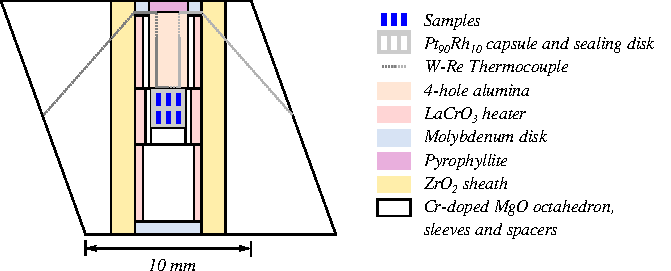
\includegraphics[width=0.8\textwidth]{figures/assembly}
  \caption{The 18/11 octahedral assembly design used in this study.}
  \label{fig:assembly}
\end{figure}

\begin{landscape}
\begin{table}[ht!]
\caption{Experimental run conditions and run products determined by SEM/EDS. Compositions are listed in order of increasing molar H$_2$O content. Unused compositions for each run are marked by an en-dash. Minor solids are listed in brackets. Mineral abbreviations are as follows: br - brucite, per - periclase, co - hydroxychondrodite, en - clinoenstatite, s - stishovite.}
\label{table:experiments}
\begin{tabular}{llllccccc}
Expt \# & P (GPa) & T ($^{\circ}$C) & t (min) & brucite+PtAc & forsterite+PtAcid & enstatite+PtAcid & quartz+PtAcid & br+q \\
Z1063 & 13 & 1200 & 40 & -/br/br/br/L & co/fo/fo/(fo) & en/en/en/en & -/-/-/-/-/-/-/- & -/-/-/- \\
Z1085 & 13 & 1300 & 40 & -/-/per/L/L & -/fo/(en)/L & -/-/-/- & -/-/-/-/-/-/-/- & -/-/-/- \\
Z1079 & 13 & 1300 & 35 & -/per/per/L/L & fo/fo/en/(en) & en/en/en/en & -/-/-/-/-/-/-/- & -/-/-/- \\
Z1058 & 13 & 1400 & 30 & -/per/(per)/L/L & fo/(fo)/L/L & en/en/en/(en) & -/-/-/-/-/-/-/- & -/-/-/- \\
Z1060 & 13 & 1500 & 20 & -/-/-/-/- & (fo)/L/L/L & en/en/L/L & -/-/-/-/-/-/-/- & -/-/-/- \\
Z1140 & 13 & 1600 & 10 & -/-/-/-/- & -/-/-/- & -/-/-/- & s/s/s/s/s/s/s/(s) & s+en/en/en/en \\
Z1084 & 13 & 1650 & 10 & -/-/-/-/- & -/-/-/- & L/L/-/- & -/-/-/-/-/-/-/- & -/-/-/- \\
Z1207 & 13 & 1700 & 8 & -/-/-/-/- & -/-/-/- & -/-/-/- & s/s/s/s/s/s/(s)/L & s+en/(en)/L/L \\
Z1209 & 13 & 1800 & 5 & -/-/-/-/- & -/-/-/- & -/-/-/- & s/s/s/s/(s?)/L/L/L & s/L/L/L \\
Z1091 & 13 & 1900 & 5 & (per)/-/-/-/- & -/-/-/- & -/-/-/- & -/-/-/L/-/L/L/L & L/L/-/-
\end{tabular}
\end{table}
\end{landscape}


\begin{figure}[ht!]
  \centering
      %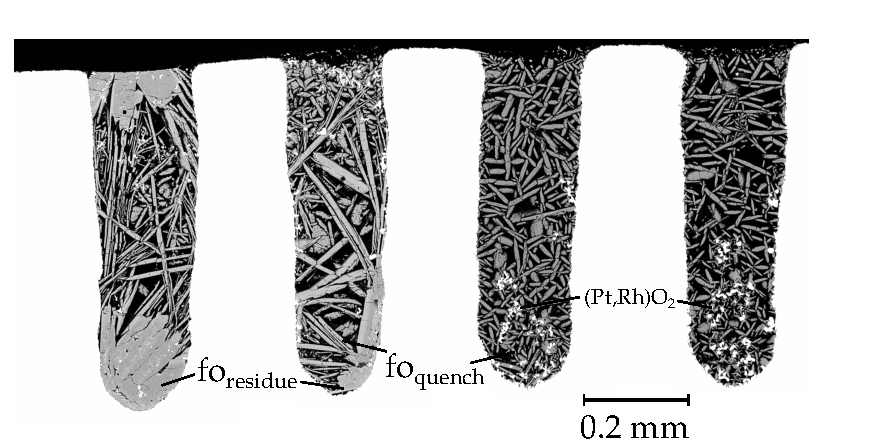
\includegraphics[width=0.8\textwidth]{figures/Z1058_1400C_13GPa_fo}
  \caption{BSE image of typical run products. Experimental chambers from Experiment Z1058, conducted at 1400 $^{\circ}$C and 13 GPa. Chambers have compositions along the forsterite-water binary, with water contents increasing from left to right.}
  \label{fig:sem}
\end{figure}


\subsection{Subsystems}
\subsubsection{MgO-H$_2$O}
Experimental results for the system MgO-H$_2$O are shown in Figure \ref{fig:MH}. The periclase-brucite-water invariant at 13 GPa is well constrained at 62--66 mol\% H$_2$O and $\sim$1200 $^{\circ}$C. The MgO content of the fluid increases gradually with increasing pressure, as a result of the extremely high melting temperature of periclase. In addition to the thermodynamic models described in the methods section, the activity of H$_2$O at the brucite-periclase-melt triple point is calculated using the thermodynamic dataset of \citep{HP2011}, which includes models for brucite, periclase and water \citep{PS1995}. This provides an additional constraint on the melt model via the equation
\begin{equation}
RT \ln a_{H_2O} =  G_{br} - G_{per} - G_{H_2O}
\end{equation}
The brucite melting curve is obtained by finding the solution to the equation
\begin{equation}
(G_{MgO, melt} + RT \ln a_{MgO}) + (G_{H_2O, HP} + RT \ln a_{H_2O}) = G_{br, HP} - G_{per, HP} + G_{per, SLB}
\end{equation}
\noindent where the right hand side is the chemical potential of Mg(OH)$_2$ in the melt, and the right hand side is the Gibbs free energy of brucite with a correction for the different standard state energies of MgO between the \cite{HP2011} and \cite{SLB2011} datasets. $G_{(1)} = RT \ln K_{(1)} = -75000$ J/mol ($r$=1) provides a good fit to the data if additional asymmetry is added via a binary subregular model (W$_{MgO-H_2O}$=55000 J/mol, W$_{H_2O-MgO}$=0 J/mol). The large positive interaction parameter increases the tendency for melt-fluid immiscibility at the water-rich end of the system. This is reflected in the flat slope of the brucite liquidus, and is in excellent agreement with the suggestion that the second critical endpoint in the MgO-H$_2$O system probably lies at ca. 12--13 GPa \citep{MSUP2007}.

\begin{figure}[ht!]
  \centering
      %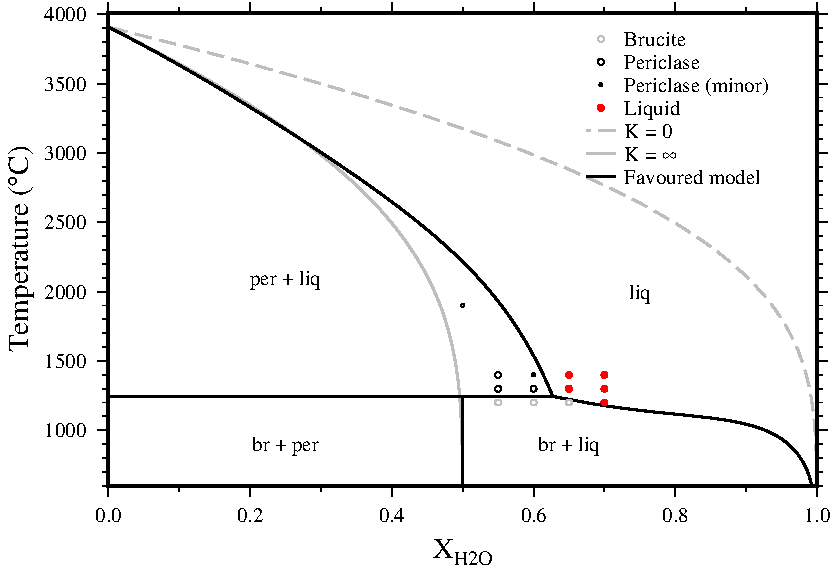
\includegraphics[width=0.8\textwidth]{figures/periclase}
  \caption{The periclase-water phase diagram at 13 GPa, based on current experimental results. Model fits to the data use the melt formulation of \cite{SS1985}, with r=1 and K=K(T) (see discussion in main text). Properties of the anhydrous solid and melt are taken from published literature \citep{SLB2011, DKS2013}. An additional subregular interaction term is required to match the composition and temperature of brucite dehydration.}
  \label{fig:MH}
\end{figure}



The dehydration of brucite at high pressure was previously studied by \cite{FIYKFO2005}. They reported that the stability of brucite reaches a maximum at about 9--10 GPa and 1200 $^{\circ}$C, decomposing at 1100--1150 $^{\circ}$C at 13 GPa. The temperature difference between their study and ours is therefore 50 $^{\circ}$C, within experimental uncertainties. 


\clearpage
\subsubsection{Mg$_2$SiO$_4$-H$_2$O}
The melting point depression of forsterite in the presence of water at 13 GPa is illustrated in Figure \ref{fig:foH}. The model parameters shown are $G_{(1)} = 75 \cdot (1420-T)$ J/mol, $r=4/3$. The anhydrous melting of forsterite is incongruent, so the high temperature part of the liquidus is metastable with respect to a mixture of periclase and liquid (see also Figure \ref{fig:ternary}). Water-rich chambers from experiments run at 1300 $^{\circ}$C revealed small quantities of enstatite, indicating that the forsterite-enstatite cotectic crosses the Mg$_2$SiO$_4$-H$_2$O tie line at 1300-1400 $^{\circ}$C. This is in excellent agreement with results on the wadsleyite-water system run at 15 GPa \citep{DDFK2005, LSOK2011}. At 1200 $^{\circ}$C, one chamber contained large crystals of hydroxychondrodite. The presence of this MgO-rich phase in the chamber with the lowest water contents may be explained an MgO-deficit in forsterite resulting from the incorporation of hydrogen via the substitution mechanism Mg$^{2+}$ $\rightarrow$ 2H$^+$ \citep{KB2006}. Alternatively it could simply be the result of a small SiO$_2$ deficit in that sample chamber. 

\begin{figure}[ht!]
  \centering
      %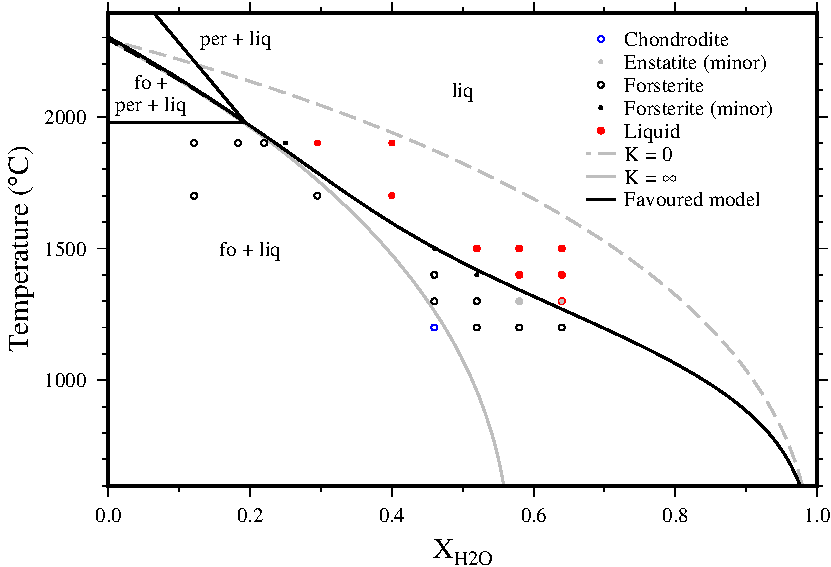
\includegraphics[width=0.8\textwidth]{figures/forsterite}
      \caption{The forsterite-water phase diagram at 13 GPa, based on current experimental results. The thermodynamics of pure forsterite are taken from the literature \citep{SLB2011}, and the properties of the anhydrous melt are from the mixing model described in the text. At high temperatures, the forsterite liquidus is metastable with respect to periclase + melt. High temperature data come from the study of \cite{NDMF2015}.}
  \label{fig:foH}
\end{figure}
\clearpage


\subsubsection{MgSiO$_3$-H$_2$O}
The melting of high pressure clinoenstatite in the presence of water is shown in Figure \ref{fig:eoH}. Unlike the forsterite or periclase liquidi, the observed depression of melting at low water contents exceeds that predicted by even the most extreme commonly-used ideal mixing model, where all oxygens in the melt are equivalent and available for protonation, and molecular H$_2$O is absent \citep{SS1985}. The liquidus at higher water contents can be fit well with model parameters $G_{(1)} = 120 \cdot (1750-T)$ J/mol, $r=3/2$. The disagreement between this model and the experimental observations is small, and could plausibly be due to experimental error. However, given the results for stishovite (see next section), we feel that more complex models are required to explain the depression of melting in the MgSiO$_3$ system. 

\begin{figure}[ht!]
  \centering
      %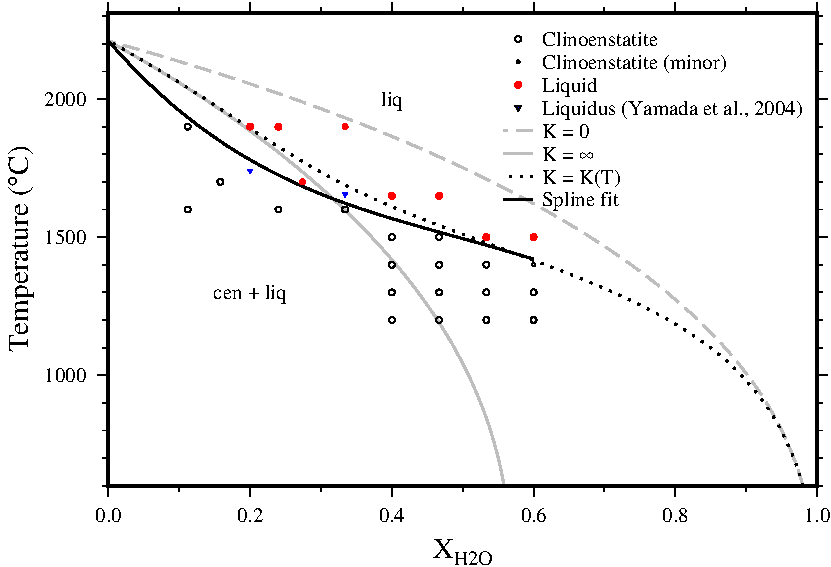
\includegraphics[width=0.8\textwidth]{figures/enstatite}
  \caption{The clinoenstatite-water phase diagram at 13 GPa, based on current experimental results. The thermodynamics of pure high pressure clinoenstatite are taken from the literature \citep{SLB2011}, and the properties of the anhydrous melt are from the mixing model described in the text. High temperature data come from the study of \cite{NDMF2015}.}
  \label{fig:eoH}
\end{figure}

Our experimentally determined liquidus is in excellent agreement with the experimental results of \cite{YII2004}, as is the absence of stishovite in any of the sample chambers. We note that although we do not have any evidence for melt-fluid immiscibility, the flat liquidus at ca. 1500 $^{\circ}$C causes a very rapid change from water-rich to water-poor fluids with increasing temperature, in agreement with \cite{Inoue1994} and \cite{YII2004}. The implication is that for a given bulk H$_2$O content, a sharp rise in the degree of partial melting will occur at about 1500 $^{\circ}$C in hydrous MgSiO$_3$ melts.

\clearpage
\subsubsection{SiO$_2$-H$_2$O}
The 13 GPa SiO$_2$-H$_2$O binary phase diagram is shown in Figure \ref{fig:SH}. While the deviation between the predicted enstatite liquidus depression for ideal molecular H$_2$O-free melts and the experimental observations are relatively small, the deviation for the stishovite data is extreme. The mixing model presented in Figure \ref{fig:SH} has parameters $G_{(1)} = 100 \cdot (1200-T)$ J/mol, $r=2$ is fit to the extrapolation of the experimentally defined liquiudus, but clearly fails to fit any of the experimental data. There are several possible explanations for this. First, the melting point of anhydrous stishovite (which is metastable with respect to coesite) could be overestimated by ca. 300 $^{\circ}$C, or the entropy of melting could be 10--20 J/K/mol, rather than 40 J/K/mol. Neither of these possibilities is very likely; the coesite and stishovite melting curves provide good constraints on the volume and entropy of SiO$_2$ melt in the region of the triple point at ca. 13.5 GPa. A third possibility is that approximately 30\% volume liquidus-phase stishovite crystals were missed during SEM analysis. This is also extremely unlikely; the equant and dendritic morphologies of liquidus and quench stishovite are instantly recognisable, and the thermal gradients in the capsule lead to melt separation on the timescales of the experiments, such that even a small (5\%) volume proportion of solids should be detected.

\begin{figure}[ht!]
  \centering
      %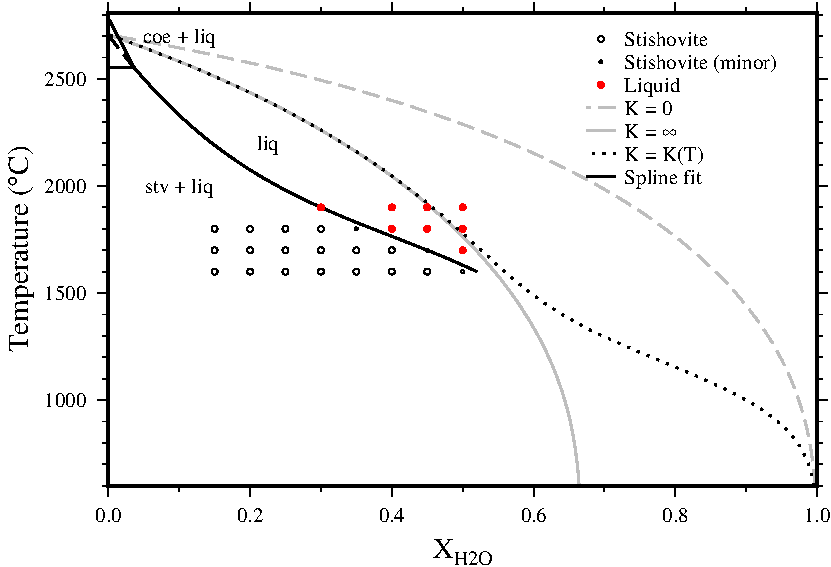
\includegraphics[width=0.8\textwidth]{figures/stishovite}
      \caption{The silica-water phase diagram at 13 GPa, based on current experimental results. The thermodynamics of stishovite and the anhydrous melt are described in the text. At high temperatures, the stishovite liquidus is metastable with respect to coesite and melt.}
  \label{fig:SH}
\end{figure}

Having ruled out experimental error and uncertainties in the thermodynamics of the anhydrous system, the only possibility is that hydrous SiO$_2$ melts with relatively low water contents are stabilised well beyond the expected entropic stabilisation from random protonation of the silica network. The causes of this additional stability (and, to a lesser extent, that of hydrous MgSiO$_3$ melts) are well beyond the scope of the current study, but may be a fruitful line of investigation for molecular dynamics simulations \citep[e.g.][]{KS2010}.

%\citep{SU2001, KOM2005, AA1980, Wunder1998, AFRH2001, Nagano2002, MFY2002, Sta2004, MFY2004, SUTG2001, NM2008, DM2010, ZK1998}

\clearpage
\subsection{The MgO-SiO$_2$-H$_2$O system}
The set of experimental analyses can be used to create a preliminary ternary liquidus diagram (Figure \ref{fig:ternary}). It should be noted that the periclase liquidus field and periclase-forsterite cotectic are poorly constrained by the data. The low temperature extension of the cotectic is chosen to fit the reported Mg:Si ratios of melts in equilibrium with forsterite and various DHMS phases at 13.5 GPa \citep{MSUP2007}. 

% Yamada et al. Figure 6 breaks Schreinemakers rules at high water contents... no reason to mention this in text, though...
 
\begin{figure}[ht!]
  \centering
      %\includegraphics[width=0.8\textwidth]{figures/experimental-ternary}
  \caption{A preliminary ternary liquidus diagram at 13 GPa, based on current experimental results. Contours are in $^{\circ}$C, and mineral abbreviations are liquidus fields as follows: per - periclase, fo - forsterite, en - clinoenstatite, stv - stishovite, coe - coesite, phB - phase B, br - brucite, chond - hydroxychondrodite, ice - ice VII.}
  \label{fig:ternary}
\end{figure}


\section{Discussion}
\subsection{Melting in deep subduction zones and atop the mantle transition zone}
Our melt model in the MSH system serves as a useful tool for investigating melting at high pressures in the mantle. In particular, the forsterite-enstatite cotectic implies that hydrous melts in equilibrium with depleted peridotites at typical mantle temperatures of 1500 $^{\circ}$C will contain $\sim$ 48 mol\% H$_2$O and an Mg:Si ratio of about 2 (the same as forsterite), corresponding to about 26 wt\% H$_2$O. Such compositions are far too water-rich to be neutrally buoyant relative to a forsterite + enstatite assemblage \citep{MSK2008}, and will rise through the mantle. Adding further components to the system will modify this behaviour. In particular, the addition of iron lowers anhydrous melting temperatures and increases melt densities. Thus, we cannot directly use our results to confirm or refute the viability of the water-filter model proposed by \cite{BK2003}, which requires neutrally buoyant or dense melts at the 410 km discontinuity. However, the flat liquidus curves revealed by our experiments are likely to also be observed in more natural chemical systems. The current results imply that the water contents of melts in equilibrium with forsterite and enstatite drop from 62 mol\% (34 wt\%) to around 30 mol\% (16 wt\%) between 1300 and 1700 $^{\circ}$C. For a given water content, this rapid change in composition must be balanced by a rapid increase in the mass fraction of partial melt, which could greatly enhance chances of detection by seismological or other geophysical techniques. Such large decreases in water content would also lead to large density changes; close to slabs, hydrous melts could be buoyant, while in warmer mantle of a similar composition they would be dense. This scenario might be expected to result in channelisation of hydrous melts close to the top interface of subducting slabs. Finally, large decreases in water contents are also likely to have a profound effect on melt viscosity, and may encourage reaction-infiltration instabilities encouraging melt channelisation \citep{SKA2001}.

% Densities
%\cite{MF2010}
%\cite{BK2003}
%\cite{MSK2008}


%So at least in my models there are three quantities that are important for the pattern of melt migration, the permeability, the compaction viscosity and the shear viscosity (if you have elasticity/plasticity, other things come in, too). Everywhere in the equations where you have the permeability, it's divided by the melt viscosity, and the permeability itself is normally assumed to scale with phi^3 (or less common phi^2), and at least I didn't see any parametrisations describing the effect of temperature on the permeability, so I would assume it's small. So for the permeability, you can just use the values you get for your different P-T-X conditions, and see if the overall term permeability/melt_viscosity increases or decreases.

%For the viscosities of the solid you have the influence of temperature on the viscosity (which I think is similar for shear and compaction viscosity) and you have the effect of porosity, eta ~ exp(alpa * phi) with phi~-27 for the shear viscosity (I think this is what Rich Katz uses in his models, but I would have to look it up to be sure), and xi ~ phi0/phi for the compaction viscosity, and you can do the same here, compare how they change for your different P-T-X conditions.


\subsection{Water partitioning in the mantle transition zone}
% Olivine, wadsleyite and ringwoodite

Partitioning of hydrogen between mineral and melt phases can be described using a partition coefficient D:
\begin{equation}
  D^{a/b}_{H_2O} = c^a_{H_2O} / c^b_{H_2O}
\end{equation}
where $c^i_{H_2O}$ is the concentration of H$_2$O (in wt\%) in phase $i$ \citep{KB2006}. In quenchable phases, there are a number of ways that concentration can be measured, including FTIR, SIMS and ERDA. In the case of melts, which are unquenchable, $c^{melt}_{H_2O}$ in partitioning studies has most commonly been estimated by mass balance or by assuming that the deficit in microprobe totals is due to hydrogen. In two studies on Fe-free wadsleyite, \cite{DDFK2005} and \cite{LSOK2011} present estimates of water content in melts calculated from microprobe deficits. A similar study on ringwoodite was undertaken by \cite{OMY2000}. The T-X$_{H_2O}$ dependencies of the melts in equilibrium with wadsleyite or ringwoodite are strikingly different (Figure \ref{fig:fo_wad_rw_melt}). For example, melt in equilibrium with wadsleyite at 15 GPa and 1400 $^{\circ}$C was estimated to contain 10.6-13.3 wt\% H$_2$O, while melt compositions in equilibrium with ringwoodite at 20 GPa and 1400 $^{\circ}$C suggest water contents of 57-66 wt\% H$_2$O. Modelled Mg$_2$SiO$_4$ melting temperatures increase by only 40 K between 15 and 20 GPa, and entropies of melting at these two pressures are not very different (92.4 vs. 97 J/K/mol), so unless the thermodynamics of mixing in the liquid change markedly between these pressures, estimates of $c^{melt}_{H_2O}$ for the ringwoodite or wadsleyite studies (or both) must be somewhat inaccurate. We note that two of the three melt compositions in equilibrium with ringwoodite fall above the temperatures indicating that hydrogen exists only as molecular H$_2$O \citep{SS1985}. In addition, the calculated liquidus temperatures in the wadsleyite studies at 15 GPa are lower than those reported at 5.5 GPa \citep{Inoue1994}. Both of these observations appear highly unlikely.

Here, we recalculate the wadsleyite/melt and ringwoodite/melt partitioning values with our melt model, assuming that our fitted values of $G_{(1)}$ and $r$ are suitable between 13 and 20 GPa. We justify this by noting that speciation is likely to be only weakly dependent on pressure under these conditions. Water concentrations in the solid are taken from the original studies. We restrict our analysis to data from 1100--1400 $^{\circ}$C, where the Mg:Si ratios of the melts are similar to that in forsterite. At 15 GPa, $D^{wad/melt}_{H_2O}$ increases from 0.30 to 0.51 between 900 and 1200 $^{\circ}$C, and then decreases back to 0.32 at 1400 $^{\circ}$C. The three ringwoodite H$_2$O concentrations (20-23 GPa) indicate a decrease in $D^{rw/melt}_{H_2O}$ from 0.68 to 0.57 between 1300 and ca. 1400 $^{\circ}$C.

\begin{figure}[ht!]
  \centering
      %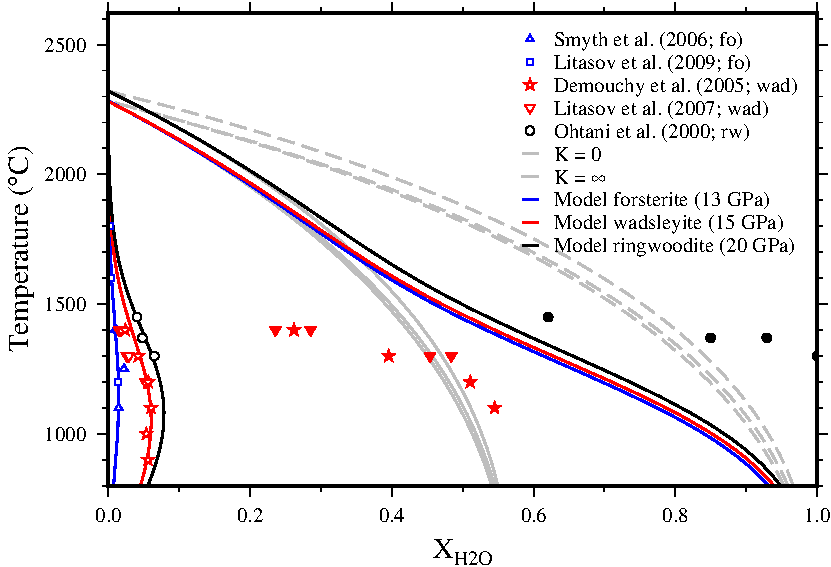
\includegraphics[width=0.8\textwidth]{figures/fo_wad_rw}
  \caption{Water concentrations in wadsleyite, ringwoodite and melt, modelled at 15 and 20 GPa. Experimental data is taken from three published studies \citep{OMY2000,DDFK2005,LSOK2011}.}
  \label{fig:fo_wad_rw_melt}
\end{figure}

We now create thermodynamic models for incorporation of H$_2$O into forsterite, wadsleyite and ringwoodite. For forsterite, we use high pressure (12--14 GPa) experimental data on the solids from \cite{SFNHB2006} and \cite{LSKO2009}; neither of these studies estimate coexisting melt compositions. Hydrogen in all three minerals is incorporated as proton pairs substituting for Mg (Mg$^{2+}$ $\leftrightarrow$ 2H$^{+}$) \citep{Smyth1987, SHFJLM2003}. Ringwoodite potentially also exhibits a substitution involving Si (Si$^{4+}$ $\leftrightarrow$ Mg$^{2+}$ + 2H$^{+}$) \citep{KKMO2000}. Both of these reactions may be written in the form 
\begin{equation}
H_2O + O = (OH)_2
\end{equation}
which leads to the equilibrium relation 
\begin{eqnarray}
\Delta G = -R T \ln \left( \frac{a_{(OH)_2}}{a_{H_2O}a_{O}} \right), \\
= \Delta H - (T-T_0) \Delta S + (P-P_0) \Delta V
\end{eqnarray}
where $\Delta G$ is the Gibbs energy associated with the reaction. The second equation is a linearised form of the expression describing the change in free energy with pressure and temperature. The first equation can be simplified by making the approximation that $a_O$ is constant and that the weight percentage of H$_2$O in the solid $c_{H_2O}$ is proportional to the activity of (OH)$_2$. Both of these assumptions are probably reasonable at low values of $c_{H_2O}$. Rearranging now produces the expression:
\begin{equation}
c_{H_2O} \propto a_{H_2O} \exp{ \left( -\frac{\Delta H - (T-T_0) \Delta S + (P-P_0) \Delta V}{R T} \right) }
\end{equation}
Further simplifications can be made by taking $T_0 = 0$ K, by realising that $P_0$ can be neglected at high pressures, and by incorporating the factor $\Delta S/R$ into the exponential prefactor. Finally, it is recognised that the pressure and temperature dependence of the Gibbs free energy of water $G_{H_2O}$ is highly nonlinear. For this reason, we split the Gibbs free energy change of the anhydrous and hydrous solid from that of the liquid, yielding the equation \citep{KB2006}:
\begin{eqnarray}
c_{H_2O} = A a_{H_2O} f_{H_2O} \exp{ \left( -\frac{\Delta H + P \Delta V^{solid}}{R T} \right) }, \\
f_{H_2O} = \exp \left(\frac{\Delta G_{H_2O}}{RT} \right)
\end{eqnarray}

We calculate the fugacity of pure water $f_{H_2O}$ from the equation of state of \citep{PS1995}. We can now fit the values of A, $\Delta H$ and $\Delta V$ to the experimental data on forsterite, wadsleyite and ringwoodite using our melt model to provide estimates of $a_{H_2O}$. The sharp spike in olivine water concentrations at 1250 $^{\circ}$C reported by \cite{SFNHB2006} is difficult to fit with reasonable enthalpies, but we obtain good fits with the rest of their data, and those of \cite{LSKO2009}. The wadsleyite data of \cite{DDFK2005} at 1200 $^{\circ}$C and 14--17 GPa are consistent with a low pressure effect on water content, implying that $\Delta V \sim 10^{-5}$ m$^3$/mol, similar or slightly lower than estimates for olivine \citep[1.00 -- 1.06 $\cdot 10^{-5}$ m$^3$/mol][]{KKR1996, ZGK2004, MDAR2006}. A single data point at 18 GPa has much lower water contents, which would require $\Delta V \sim 1.25 \cdot 10^{-5}$ m$^3$/mol. This value is inconsistent with the large water contents at 16 and 17 GPa, and is probably unreasonable given the reported values for olivine. We therefore favour the lower estimate of $\Delta V$, and assume the same value for ringwoodite. The model values are shown in Table \ref{table:partitioning}.

\begin{table}[]
\centering
\caption{Thermodynamic models for water solubility in wadsleyite and ringwoodite}
\label{table:partitioning}
\begin{tabular}{lllll}
Phase & $P_{\textit{\tiny{ref}}}$ (Pa) & A [kg/(kgPa)] & $\Delta H_{P_{\textit{\tiny{ref}}}}$ [J/mol] & $\Delta V$ [m$^3$/mol] \\
\hline
% Olivine & 1.2e10 & 1.74e-11 & 1.70e5 & 1e-5 \\ Not a bad fit for the Zhao enthalpy
% Olivine & 1.2e10 & 5e-12 & 1.70e5 & 1e-5 \\ Zhao et al., 2004, water contents much too high
Olivine & 1.2e10 & 3.23e-12 & 1.50e5 & 1e-5 \\
Wadsleyite & 1.5e10 & 1.97e-12 & 1.60e5 & 1e-5 \\
Ringwoodite & 2.0e10 & 1.46e-12 & 2.03e5 & 1e-5 (fixed)
\end{tabular}
\end{table}


These models allow us to predict the partition coefficients of water between olivine, wadsleyite and melt at the 410 km discontinuity ($\sim$14 GPa; Figure \ref{fig:partitioning_rw_wad}), and wadsleyite, ringwoodite and melt at the 520 km discontinuity ($\sim$18 GPa; Figure \ref{fig:partitioning_rw_wad}). $D^{wad/fo}_{H_2O}$ displays a decrease from $\sim$4 at 1000 $^{\circ}$C to $\sim$1.8 at 2000 $^{\circ}$C, in good agreement with the estimates of \cite{LSOK2011} at low temperatures, but without a return to high values at high temperatures, where water contents are lower and prone to large relative errors. $D^{ring/wad}_{H_2O}$ decreases from $\sim$1.4 at 1000 $^{\circ}$C to $\sim$1.1 at 2000 $^{\circ}$C. These values imply that upwelling across both the 410 and the 520 km discontinuity will cause partial melting. Both boundaries have been associated with low seismic velocities, which may indicate zones of deep melting \citep[e.g.][]{JDH2010}. The small temperature dependence on the wadsleyite-ringwoodite partition coefficient implies that repartitioning of water during secular cooling within the mantle transition zone is likely to be more minor (and in the opposite direction) to that proposed by \cite{DDFK2005}. 

\begin{figure}[ht!]
  \centering
  %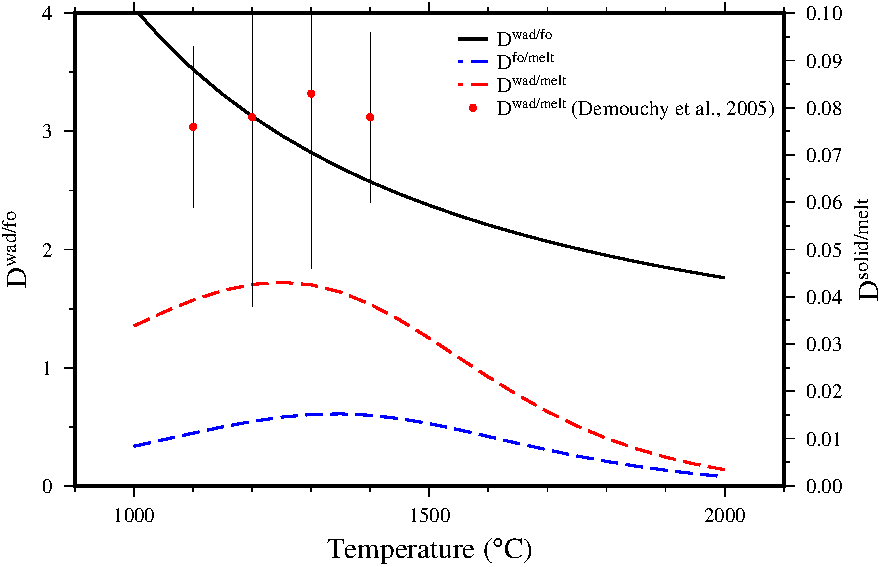
\includegraphics[width=0.8\textwidth]{figures/wad_fo_partitioning_410}
  \caption{Modelled partition coefficient between forsterite, wadsleyite and melt at 14 GPa, approximately the pressure of the 410 km discontinuity. Note the separate scales for solid/solid and solid/melt partitioning. The difference in melt compositions between this study and that of \cite{DDFK2005} results in much lower $D^{wad/melt}$ coefficients. Error bars on the wadsleyite datapoints are those reported by \cite{DDFK2005}.}
  \label{fig:partitioning_wad_fo}
\end{figure}

\begin{figure}[ht!]
  \centering
  %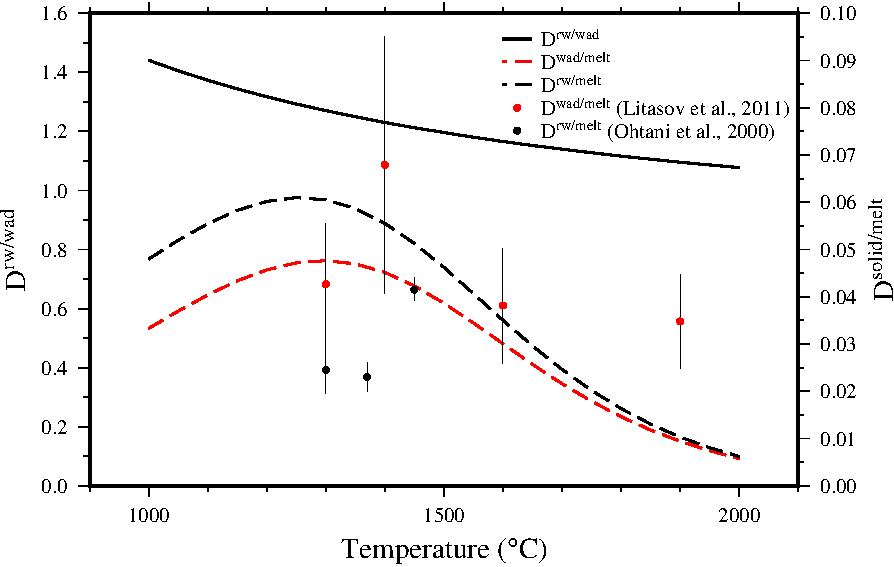
\includegraphics[width=0.8\textwidth]{figures/rw_wad_partitioning_520}
  \caption{Modelled partition coefficient between wadsleyite, ringwoodite and melt at 18 GPa, approximately the pressure of the 520 km discontinuity. Note the separate scales for solid/solid and solid/melt partitioning. Error bars on the ringwoodite data points indicate the range of values reported by \cite{OMY2000}. Error bars on the wadsleyite data points indicate 1 s.d. uncertainties as reported by \cite{LSOK2011}.}
  \label{fig:partitioning_rw_wad}
\end{figure}


\section{Acknowledgements}
The authors would like to thank Gerti Gollner for acquiring capsule materials, Stefan \"Ubelhack and Heinz Fischer for assembly and capsule cutting and Hubert Schulze for sample preparation. RM was supported by a Humboldt Postdoctoral Fellowship. This study was funded by the ACCRETE project (European Research Council Advanced Grant, contract number 290568).

\clearpage
\section*{References}

\bibliography{references_MSH}

\end{document}
